When Teststyle has been activated for a \gdproject{} \bxpref{TeststyleActivate}, you can configure:

\begin{itemize}
\item which guidelines should be used \bxpref{TeststyleActivateGuideline}
\item what kind of a message a flouted guideline should show (information, warning or error) \bxpref{TeststyleMessageLevel}
\item the attributes for a guideline \bxpref{TeststyleAttributes}
\item the contexts a guideline should be active for \bxpref{TeststyleContexts}
\end{itemize}

\subsubsection{Activating and deactivating individual guidelines}
\label{TeststyleActivateGuideline}

In the \gdproject{} properties, under the \bxname{Teststyle} section, you can activate and deactivate guidelines for use in the \gdproject{}:

\begin{enumerate}
\item When Teststyle is enabled for the \gdproject{} \bxpref{TeststyleActivate}, select the checkbox for an individual guideline to activate it for the \gdproject{}. 
\item Deselect a checkbox to deactivate the guideline. 
\bxtipp{When you select a guideline, the description text gives you more information on what the guideline is for.}
\item You can (de)select all the guidelines in a category by activating or deactivating the checkbox for the category name.
\item You can also use the buttons \bxcaption{Select All} and \bxcaption{Deselect All} to (de)select all the guidelines. 
\item Click \bxcaption{OK} in the \gdproject{} properties to save the changes.
\item If your current \gdproject{} flouts any of the guidelines that are set, then you will see entries in the \gdprobview{} notifying you of the places where guidelines are being flouted. For more information on working with the \gdprobview{} to fix tests, see the section later \bxpref{TeststyleProbView}.

\end{enumerate}


\subsubsection{Setting the message level for guidelines}
\label{TeststyleMessageLevel}

For each guideline in the \gdproject{} properties, you can decide how \app{} should notify you that the guideline is not being upheld. 

The choices available are:
\begin{description}
\item [Information:]{Information is shown in the \gdprobview{} using a blue icon. Elements in the test are not decorated with information messages.}
\item [Warning:]{Warnings are shown in the \gdprobview{} using a yellow icon. Warnings are also shown on elements in the test (e.g. \gdcases{}.}
\item[Errors:]{Errors are shown in the \gdprobview{} using a red icon. Warnings are also shown on elements in the test (e.g. \gdcases{}, \gdsuites{}. If a \gdsuite{} contains a Teststyle error, it will not be executable via the \ite{}.}
\end{description}

To set the message level for a guideline:
\begin{enumerate}
\item In the \gdproject{} properties, under the section \bxname{Teststyle}, select the guideline you want to configure.
\item In the combo-box on the right-hand side, select the level of message you want to receive if this guideline is not upheld.
\item Click \bxcaption{OK} in the \gdproject{} properties to save the changes. 
\end{enumerate}

\subsubsection{Configuring the attributes for guidelines}
\gdhelpid{testStylePropertyPageEditAttributeContextId}{Teststyle}
\label{TeststyleAttributes}

For many of the guidelines in the \gdproject{} properties, you can define the values or quantities for the aspects it checks. For example, you can edit the attribute \bxname{Maximum number of parameters} for the guideline that specifies the maximum amount of parameters on a \gdcase{}. 

To edit the attributes for a guideline:
\begin{enumerate}
\item In the \gdproject{} properties, under the section \bxname{Teststyle}, select the guideline you want to configure.
\item Click \bxcaption{Edit attributes} to open the attributes dialog.
\item In the dialog (\bxfigref{attributes}), you can see and edit the values for any editable attributes for this guideline. 
\item Confirm your changes in this dialog using \bxcaption{OK}.
\item Click \bxcaption{OK} in the \gdproject{} properties to save the changes. 
\end{enumerate}
\bxwarn{If you enter an invalid value, the default value will be used in its place.}
\begin{figure}[p]
\begin{center}
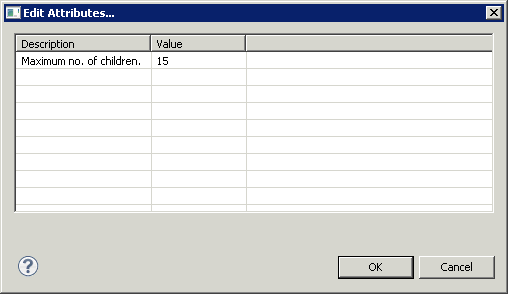
\includegraphics{Tasks/Teststyle/PS/attributes}
\caption{Edit Attributes}
\label{attributes}
\end{center}
\end{figure}


\subsubsection{Configuring the contexts for guidelines}
\gdhelpid{testStylePropertyPageEditContextContextId}{Teststyle}
\label{TeststyleContexts}

For many of the guidelines in the \gdproject{} properties, you can set the contexts they should be valid for. Some of the available contexts include \gdcases{}, \gdsuites{}, or the whole \gdproject{}. 

To edit the context for a guideline:
\begin{enumerate}
\item In the \gdproject{} properties, under the section \bxname{Teststyle}, select the guideline you want to configure.
\item Click \bxcaption{Edit context} to open the context dialog.
\item In the dialog (\bxfigref{contexts}), you can see and edit any available contexts for this guideline. 
\item To activate a context, select the checkbox next to it. To deactivate a context, deselect its checkbox.
\item Confirm your changes in this dialog using \bxcaption{OK}.
\item Click \bxcaption{OK} in the \gdproject{} properties to save the changes. 
\end{enumerate}
\bxwarn{If you enter an invalid value, the default value will be used in its place.}


\begin{figure}[p]
\begin{center}
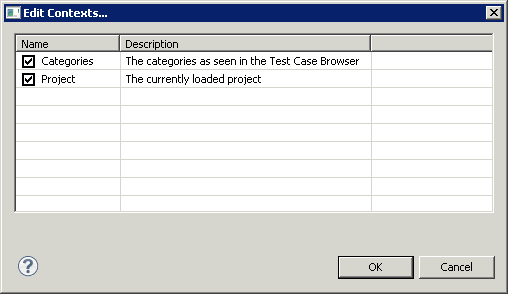
\includegraphics{Tasks/Teststyle/PS/contexts}
\caption{Edit Contexts}
\label{contexts}
\end{center}
\end{figure}
